\textcolor{black}{\section{Anexo}}

% Cambia de dos columnas a una página completa.
% También provoca el salto a la siguiente página.
\onecolumn

\thispagestyle{plain}

% =====================================================
% FILA 1
% =====================================================

\noindent
\begin{minipage}[t][0.29\textheight][t]{0.48\textwidth}
    \centering

    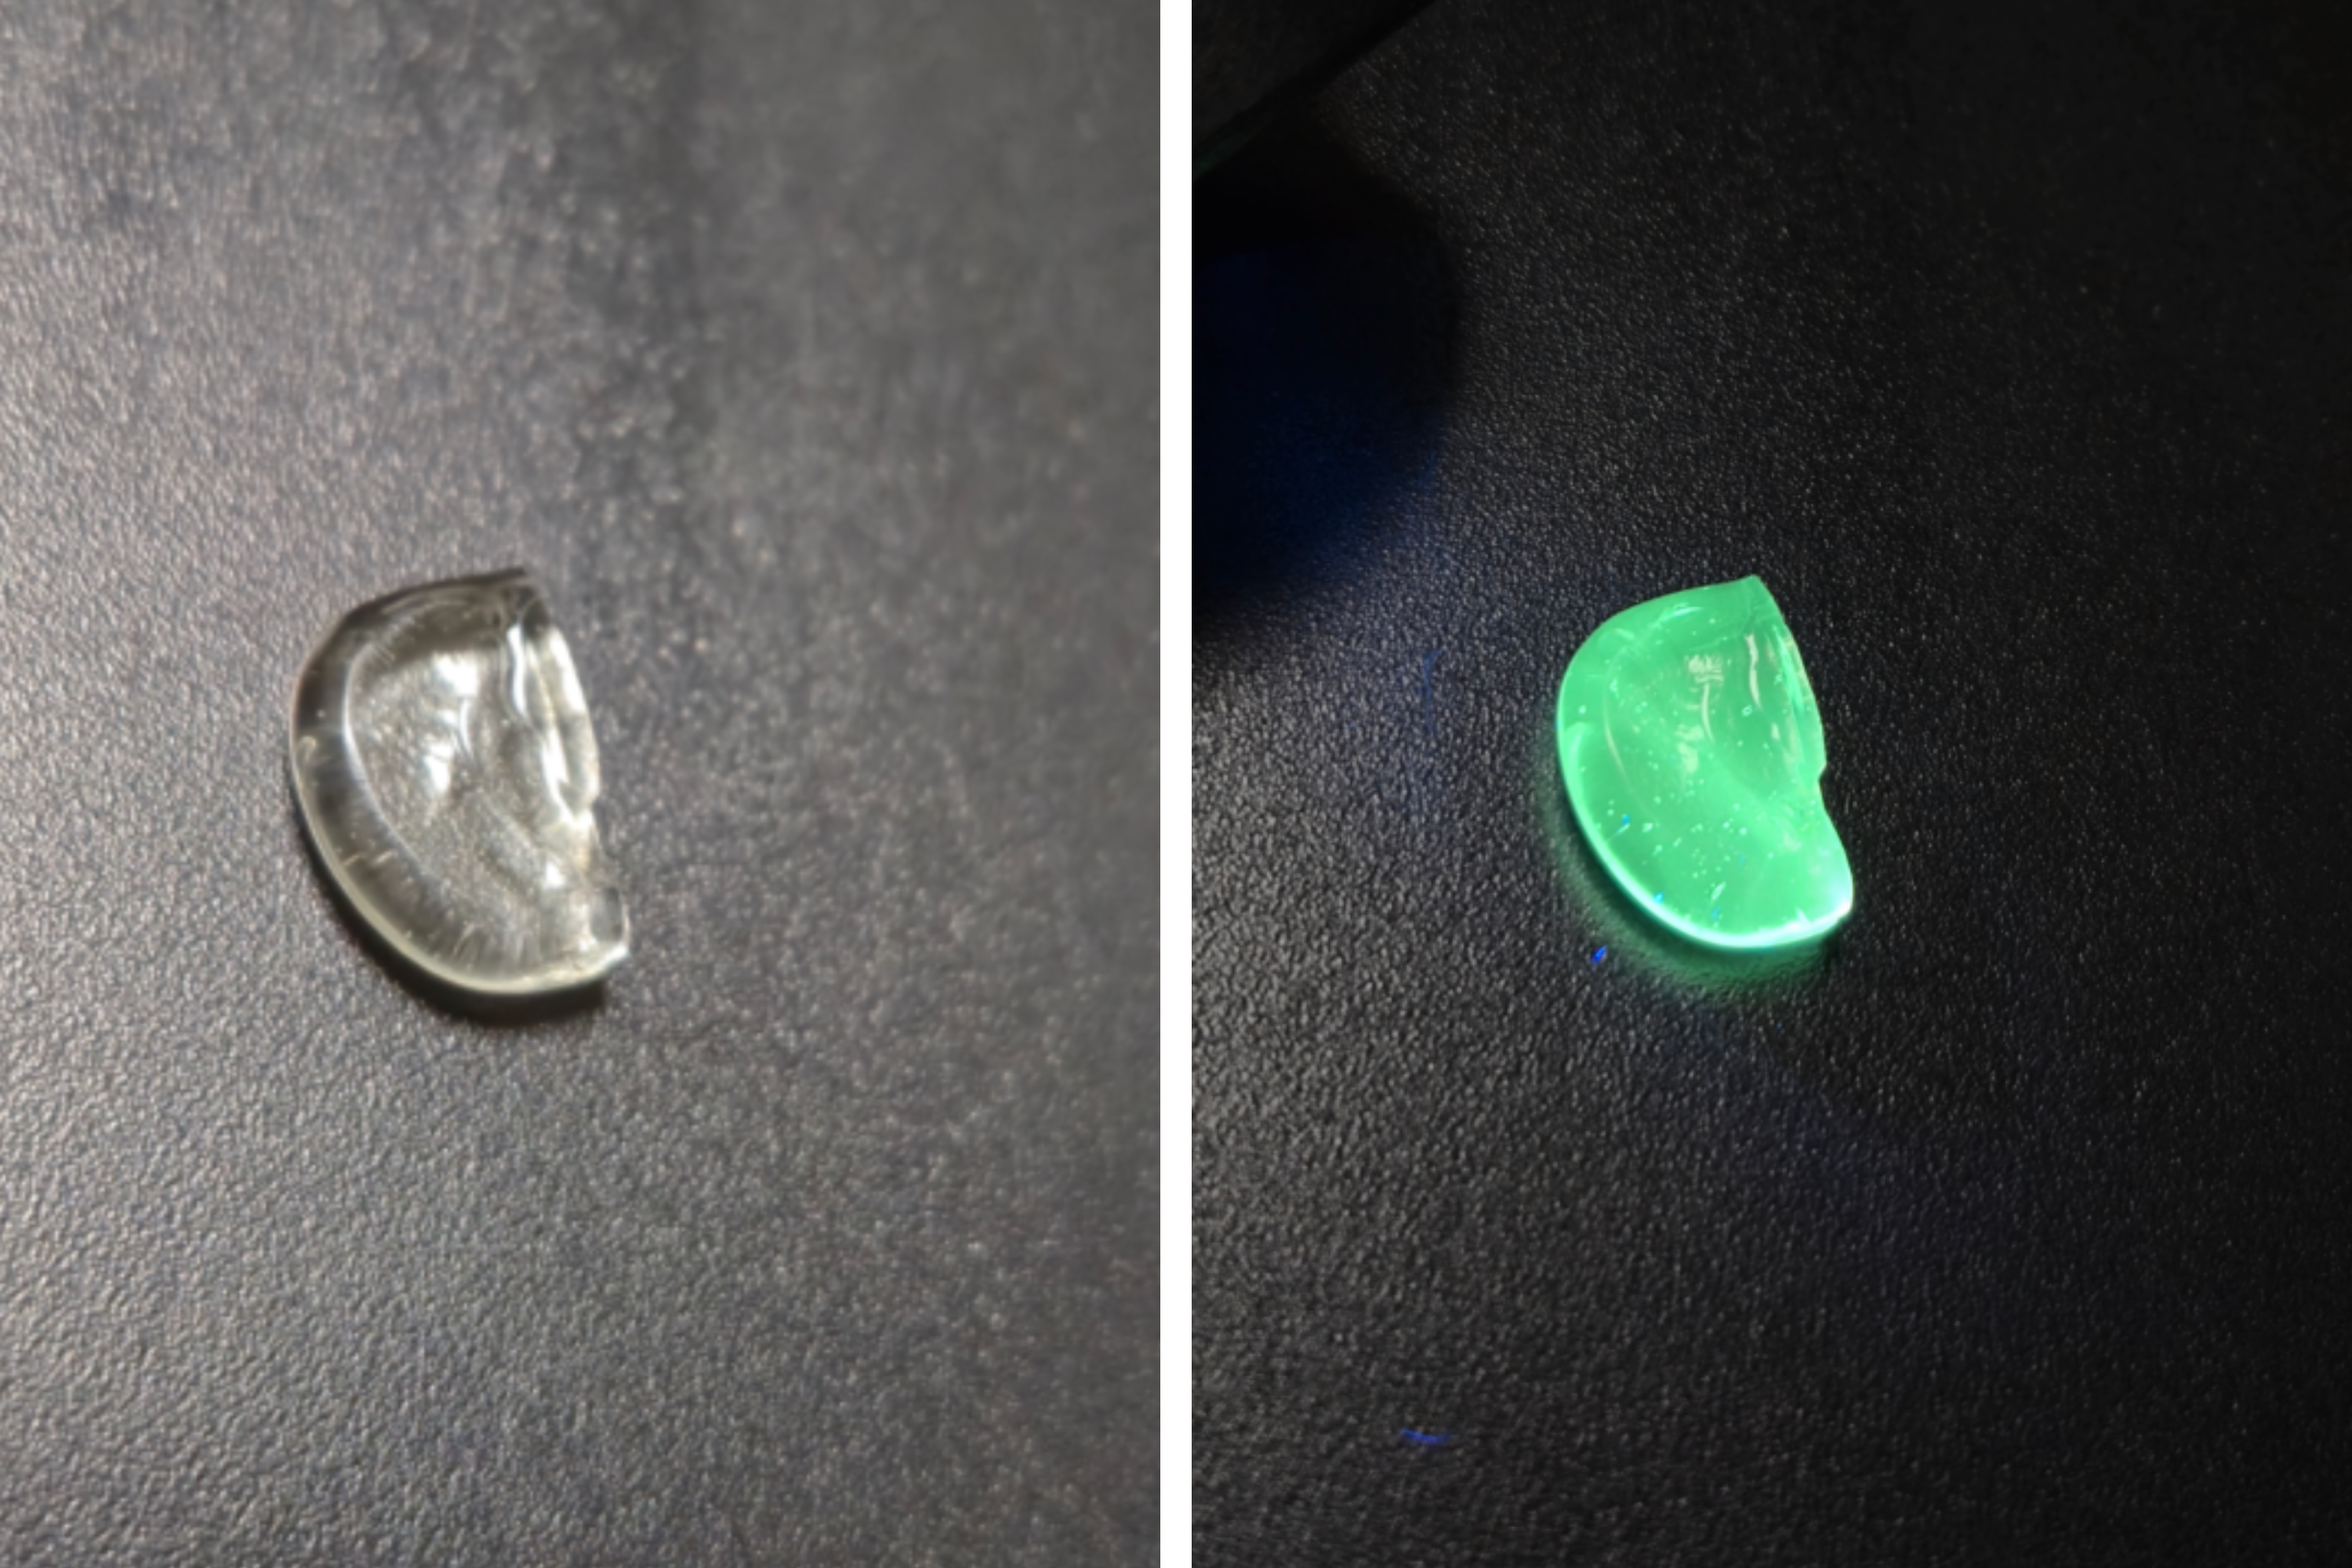
\includegraphics[
        width=\linewidth,
        height=0.22\textheight,
        keepaspectratio
    ]{figs/Dy_Mg-fotos.png}

    \captionof{figure}{
        Muestra de Mg(PO$_3$)$_2$:Mg$_3$(PO$_4$)$_2$:Dy$_2$O$_3$
        (composición molar: $49.25\%$, $49.25\%$, $1\%$).
        A la derecha presenta el fenómeno de fotoluminiscencia;
        excitado con una luz de $365$ nm.
    }
    \label{fig:Dy_Mg-fotos}
\end{minipage}%
\hfill
\begin{minipage}[t][0.29\textheight][t]{0.48\textwidth}
    \centering

    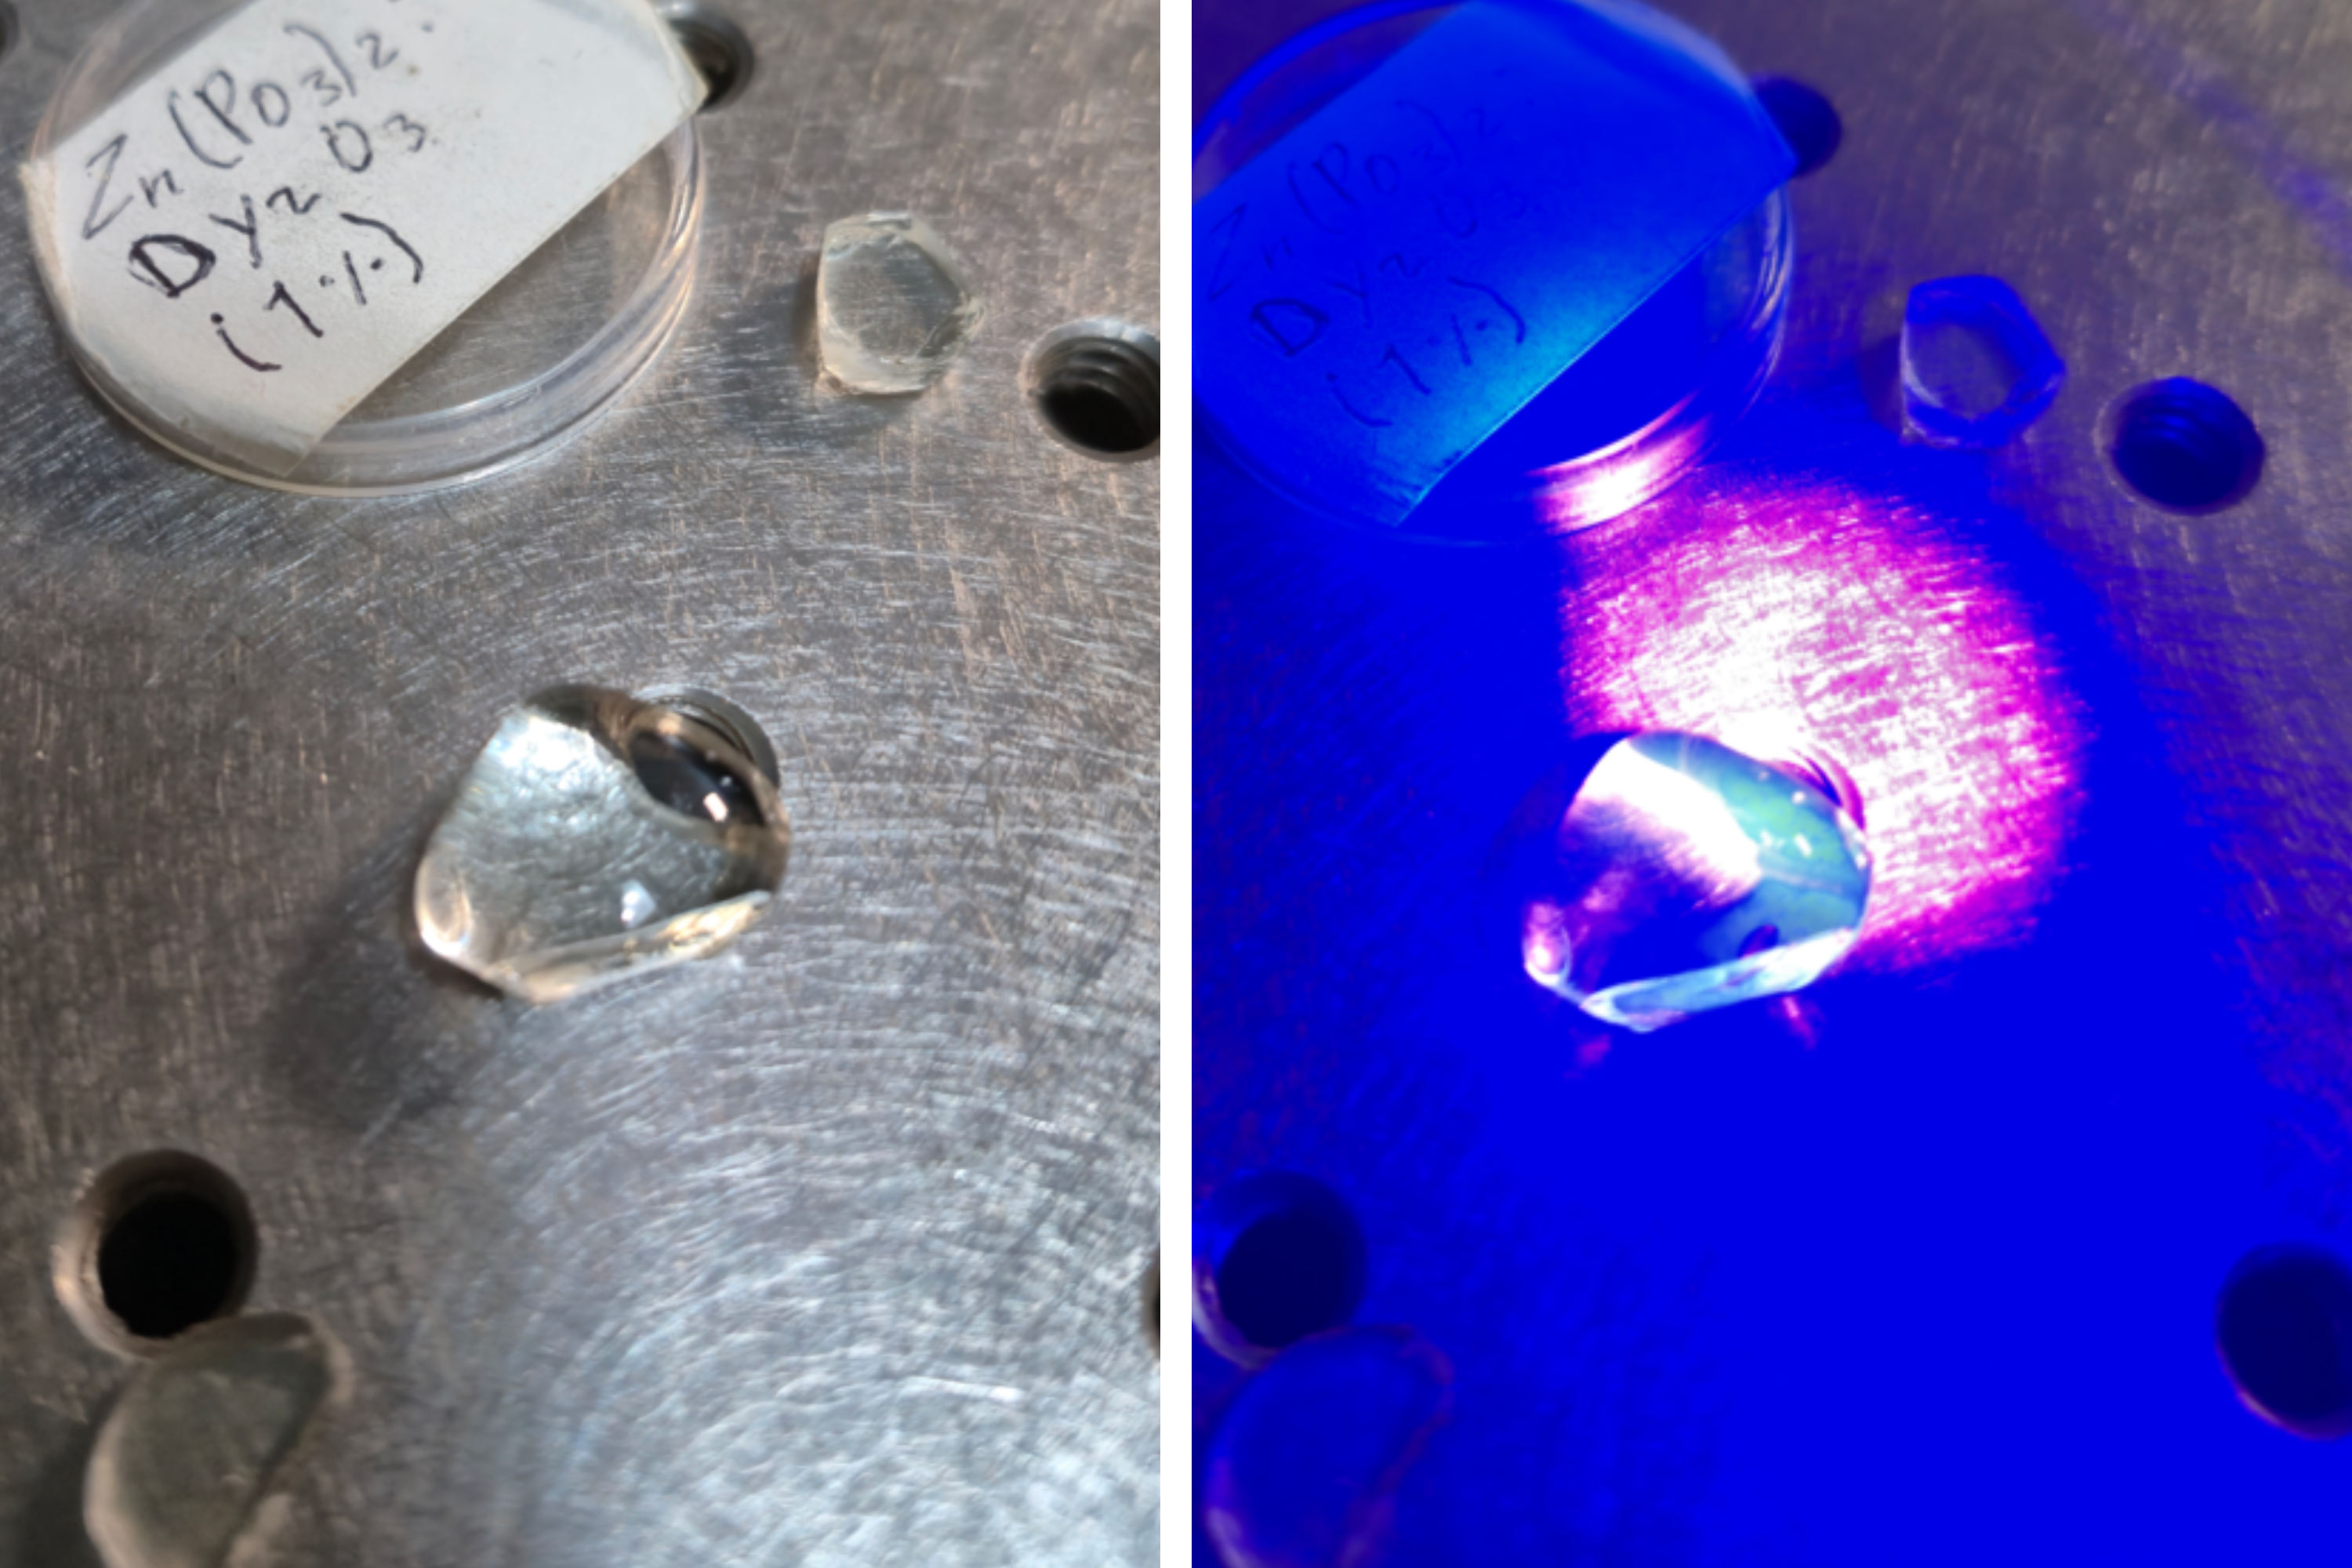
\includegraphics[
        width=\linewidth,
        height=0.22\textheight,
        keepaspectratio
    ]{figs/Dy_Zn-fotos.png}

    \captionof{figure}{
        Muestra de Zn(PO$_3$)$_2$:Dy$_2$O$_3$
        (composición molar: $99\%$, $1\%$).
        A la derecha presenta el fenómeno de fotoluminiscencia;
        excitado con una luz de $365$ nm.
    }
    \label{fig:Dy_Zn-fotos}
\end{minipage}

\vfill

% =====================================================
% FILA 2
% =====================================================

\noindent
\begin{minipage}[t][0.29\textheight][t]{0.48\textwidth}
    \centering

    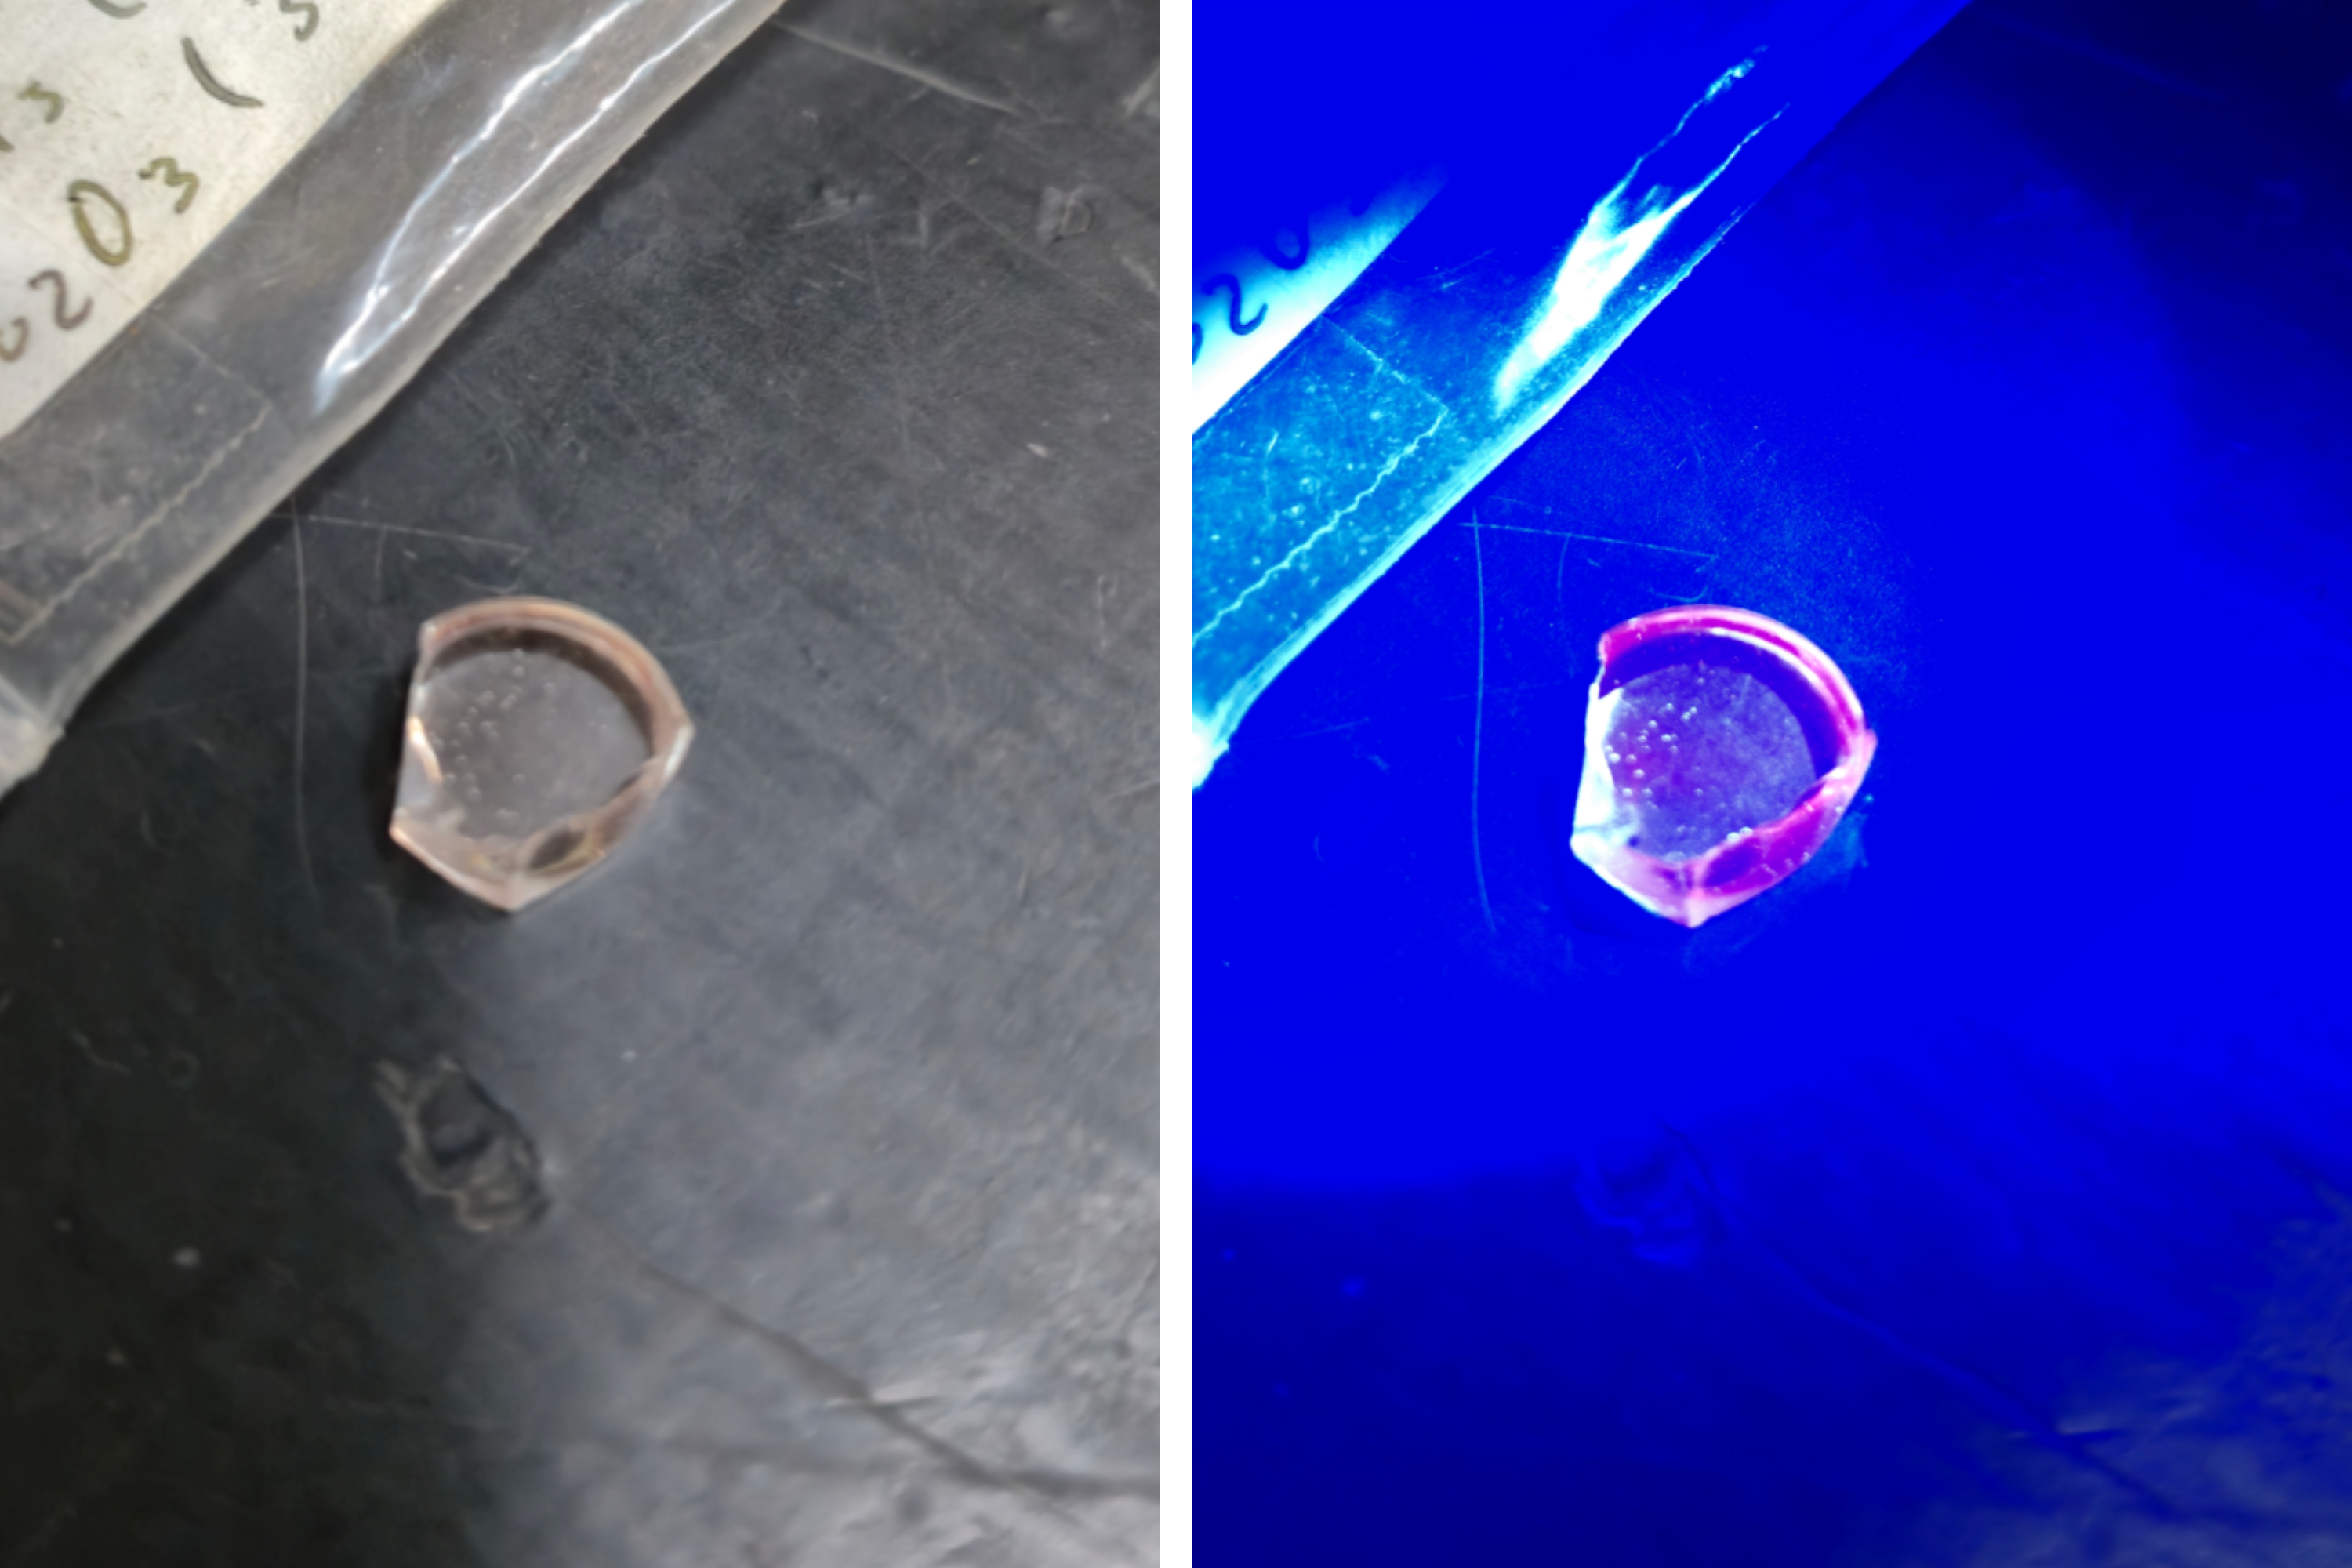
\includegraphics[
        width=\linewidth,
        height=0.22\textheight,
        keepaspectratio
    ]{figs/Eu-fotos.png}

    \captionof{figure}{
        Muestra de Mg(PO$_3$)$_2$:Mg$_3$(PO$_4$)$_2$:SnCl$_3$:Eu$_2$O$_3$
        (composición molar: $49\%$, $48\%$, $1\%$, $3\%$).
        A la derecha presenta el fenómeno de fotoluminiscencia;
        excitado con una luz de $458$ nm.
    }
    \label{fig:Eu-fotos}
\end{minipage}%
\hfill
\begin{minipage}[t][0.29\textheight][t]{0.48\textwidth}
    \centering

    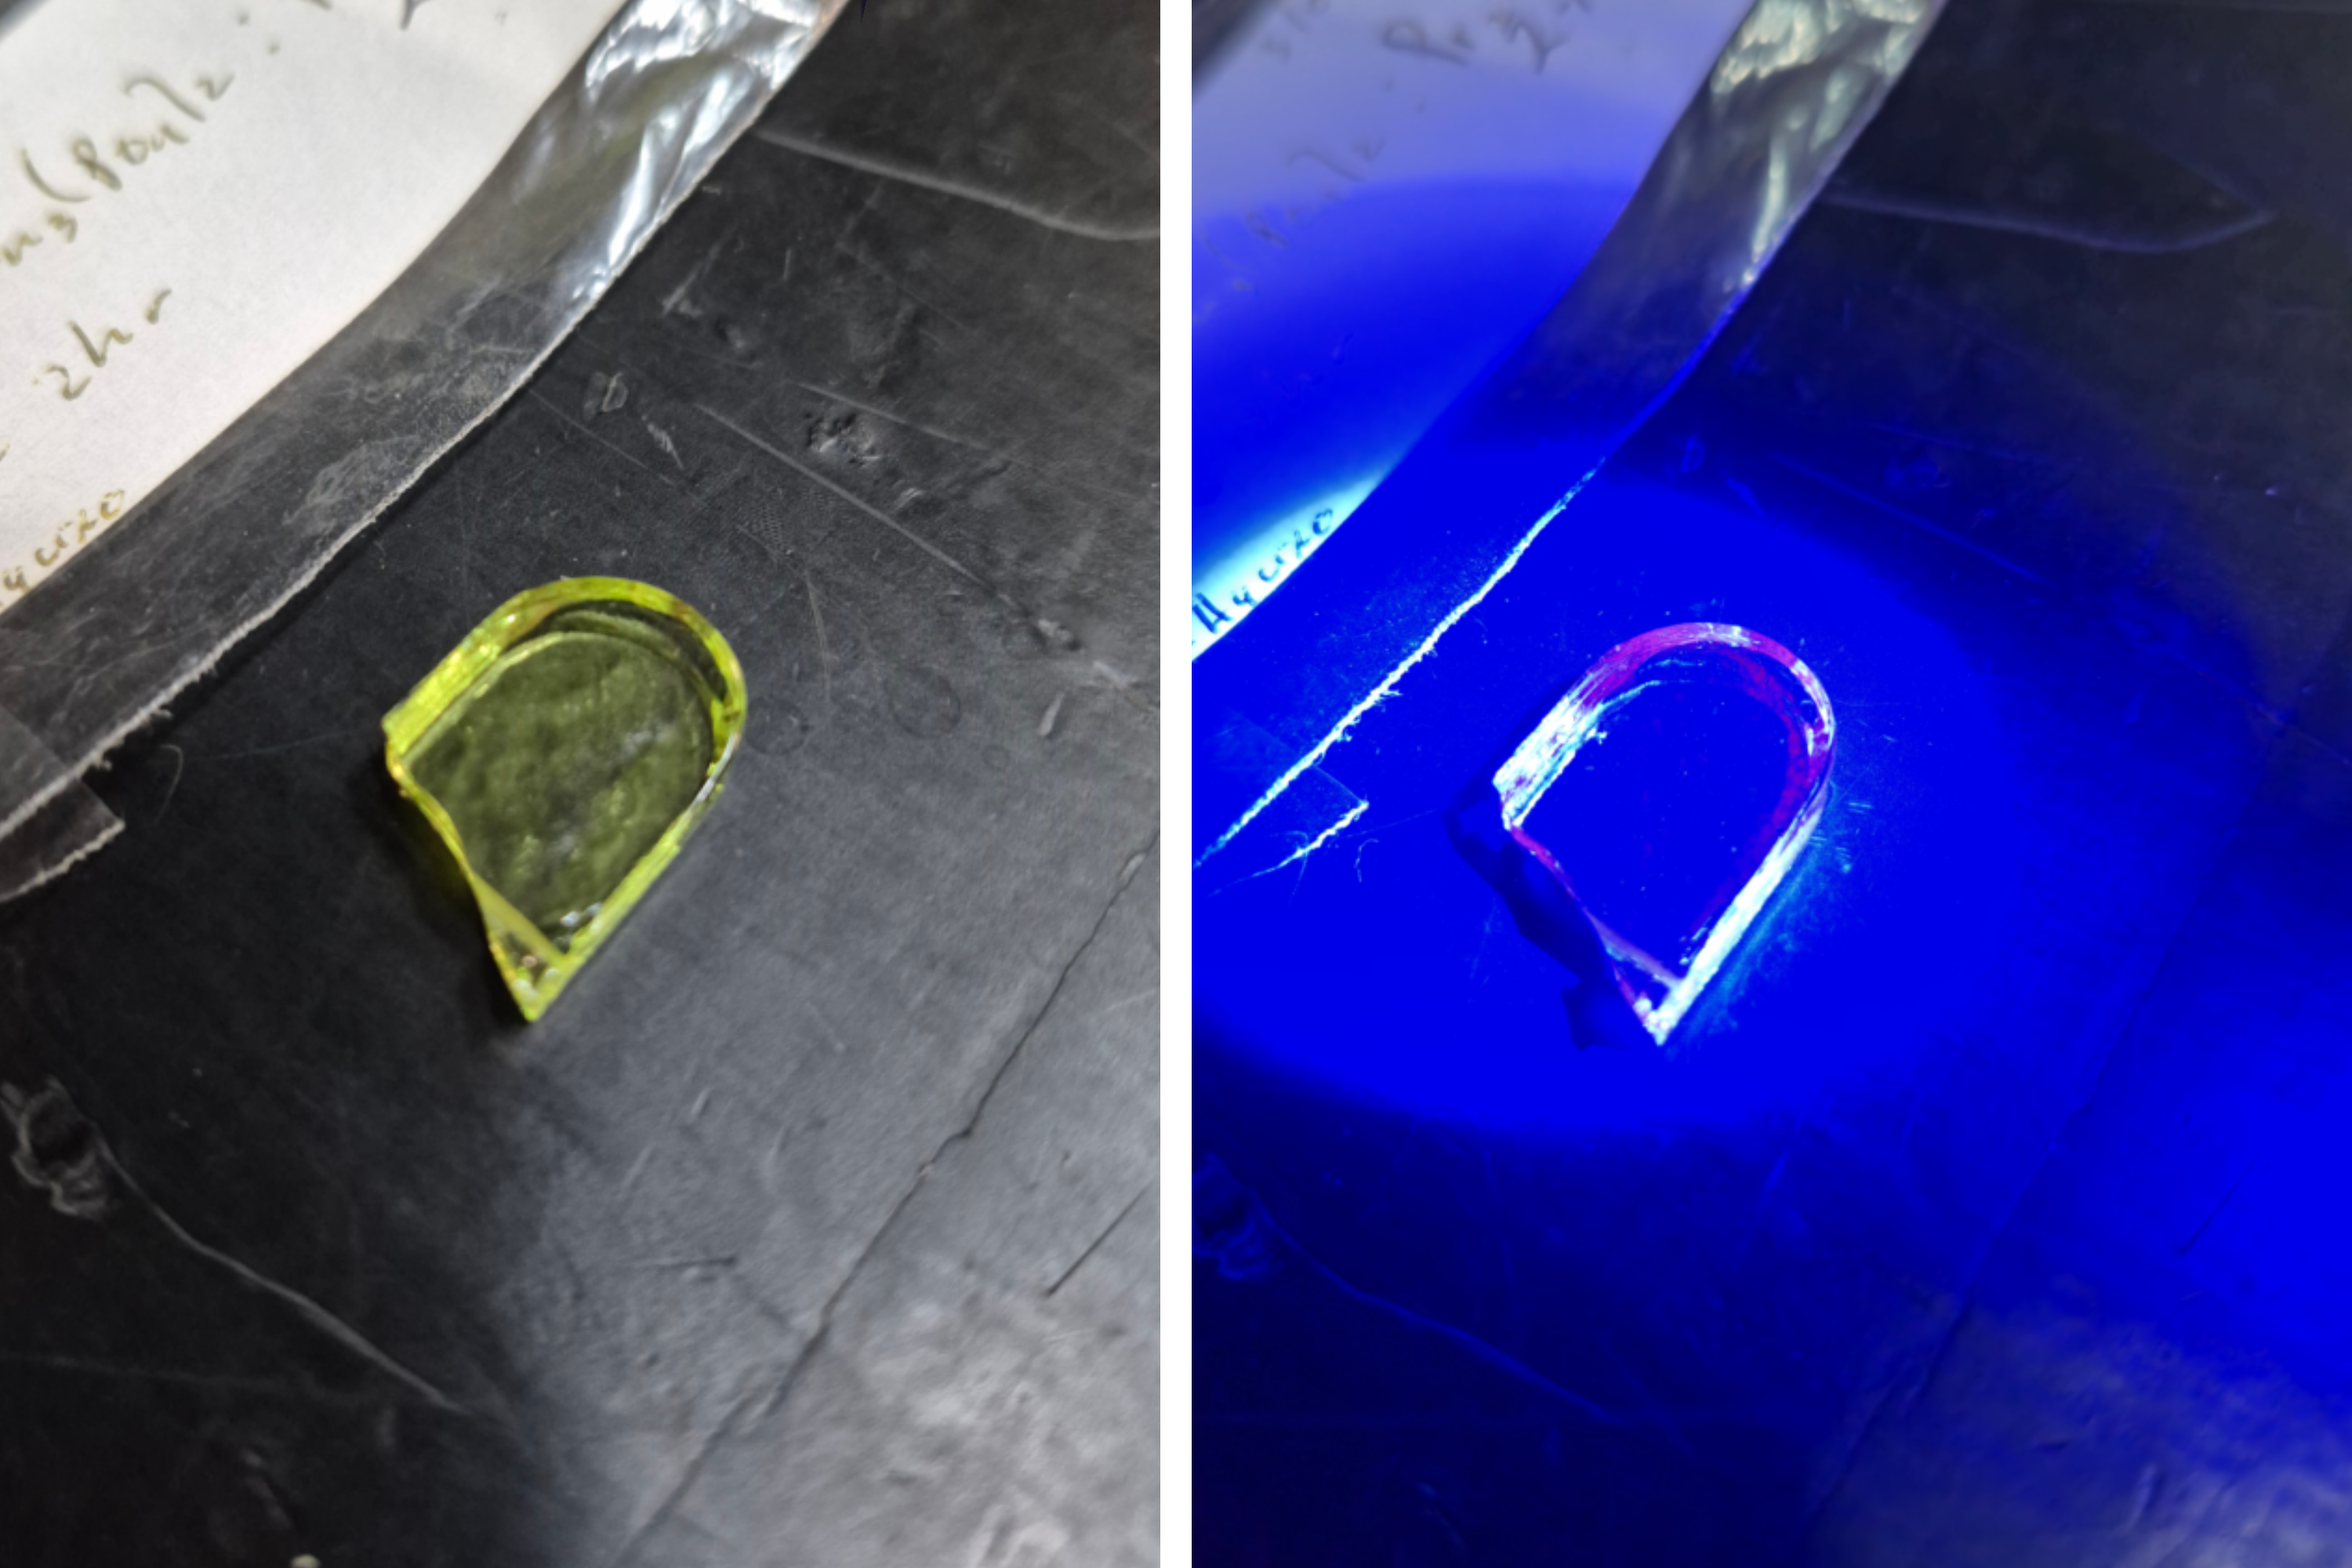
\includegraphics[
        width=\linewidth,
        height=0.22\textheight,
        keepaspectratio
    ]{figs/Pr-fotos.png}

    \captionof{figure}{
        Muestra de Zn(PO$_3$)$_2$:Zn$_3$(PO$_4$)$_2$:Pr$_2$O$_3$
        (composición molar: $49\%$, $49\%$, $2\%$).
        A la derecha presenta el fenómeno de fotoluminiscencia;
        excitado con una luz de $458$ nm.
    }
    \label{fig:Pr-fotos}
\end{minipage}

\vfill

% =====================================================
% FILA 3
% =====================================================

\noindent
\begin{minipage}[t][0.29\textheight][t]{0.48\textwidth}
    \centering

    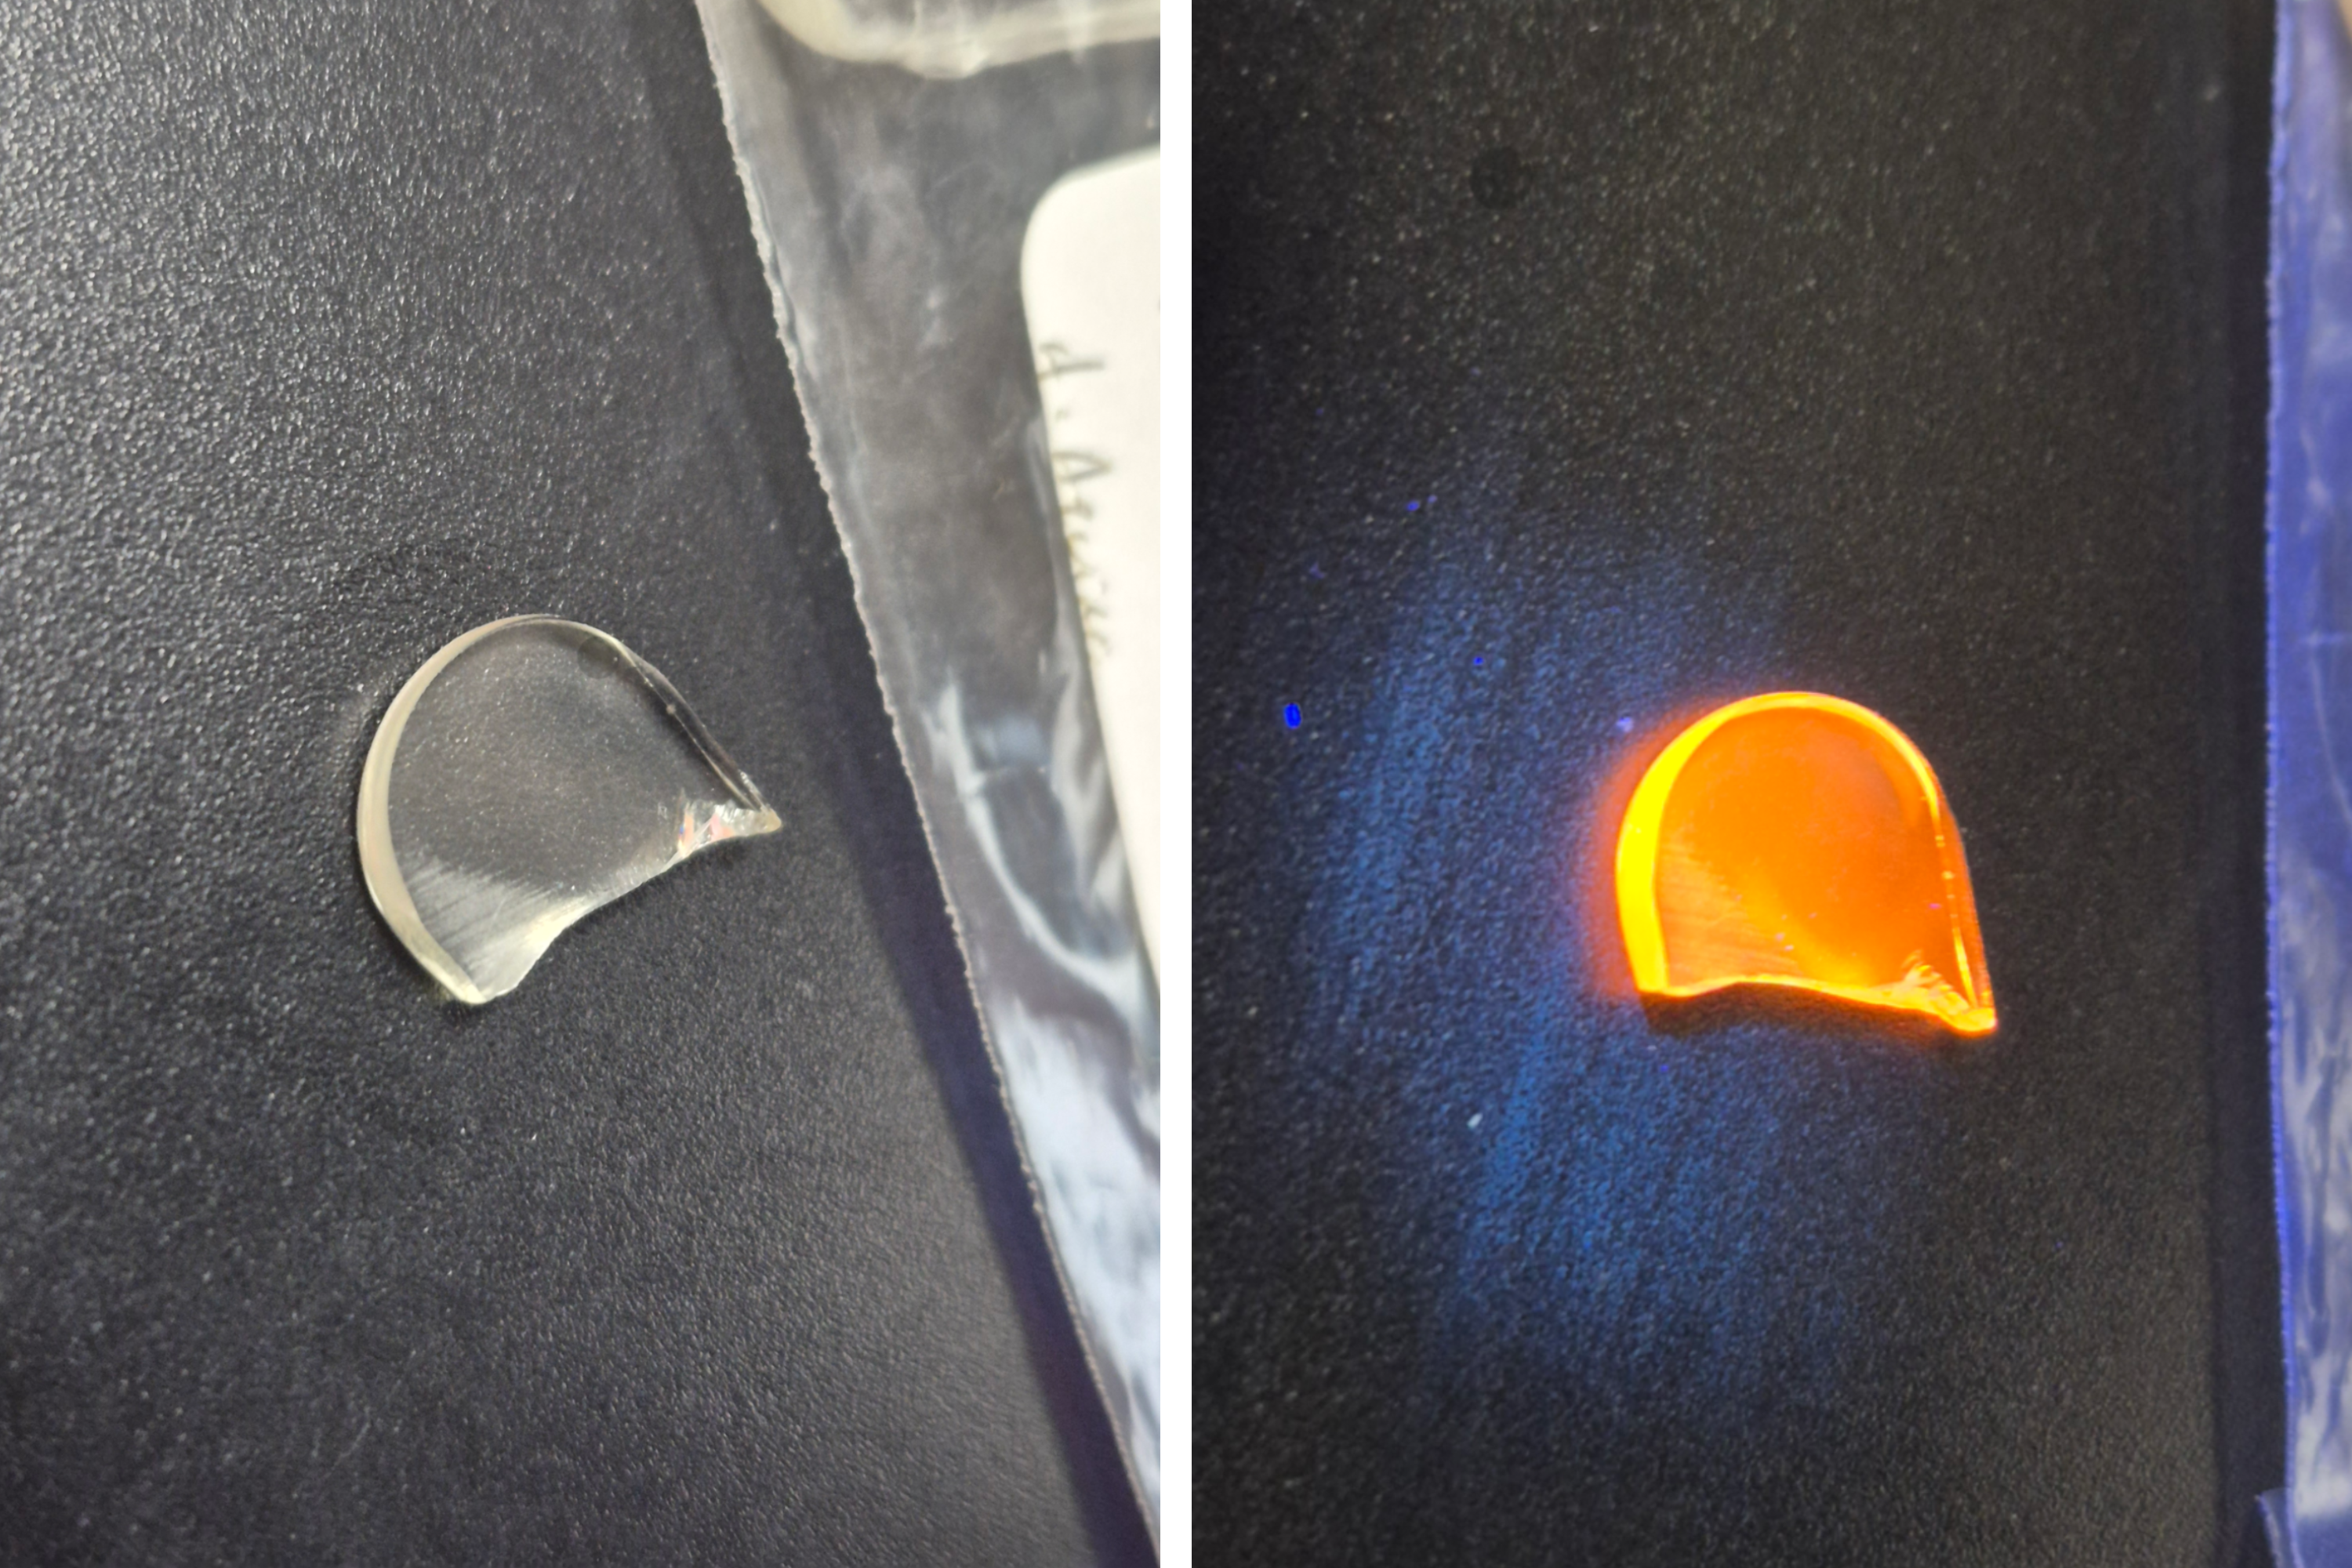
\includegraphics[
        width=\linewidth,
        height=0.22\textheight,
        keepaspectratio
    ]{figs/Sm-fotos.png}

    \captionof{figure}{
        Muestra de Zn(PO$_3$)$_2$:Zn$_3$(PO$_4$)$_2$:Sm$_2$O$_3$
        (composición molar: $49.5\%$, $49.5\%$, $1\%$).
        A la derecha presenta el fenómeno de fotoluminiscencia;
        excitado con una luz de $365$ nm.
    }
    \label{fig:Sm-fotos}
\end{minipage}%
\hfill
\begin{minipage}[t][0.29\textheight][t]{0.48\textwidth}
    \centering

    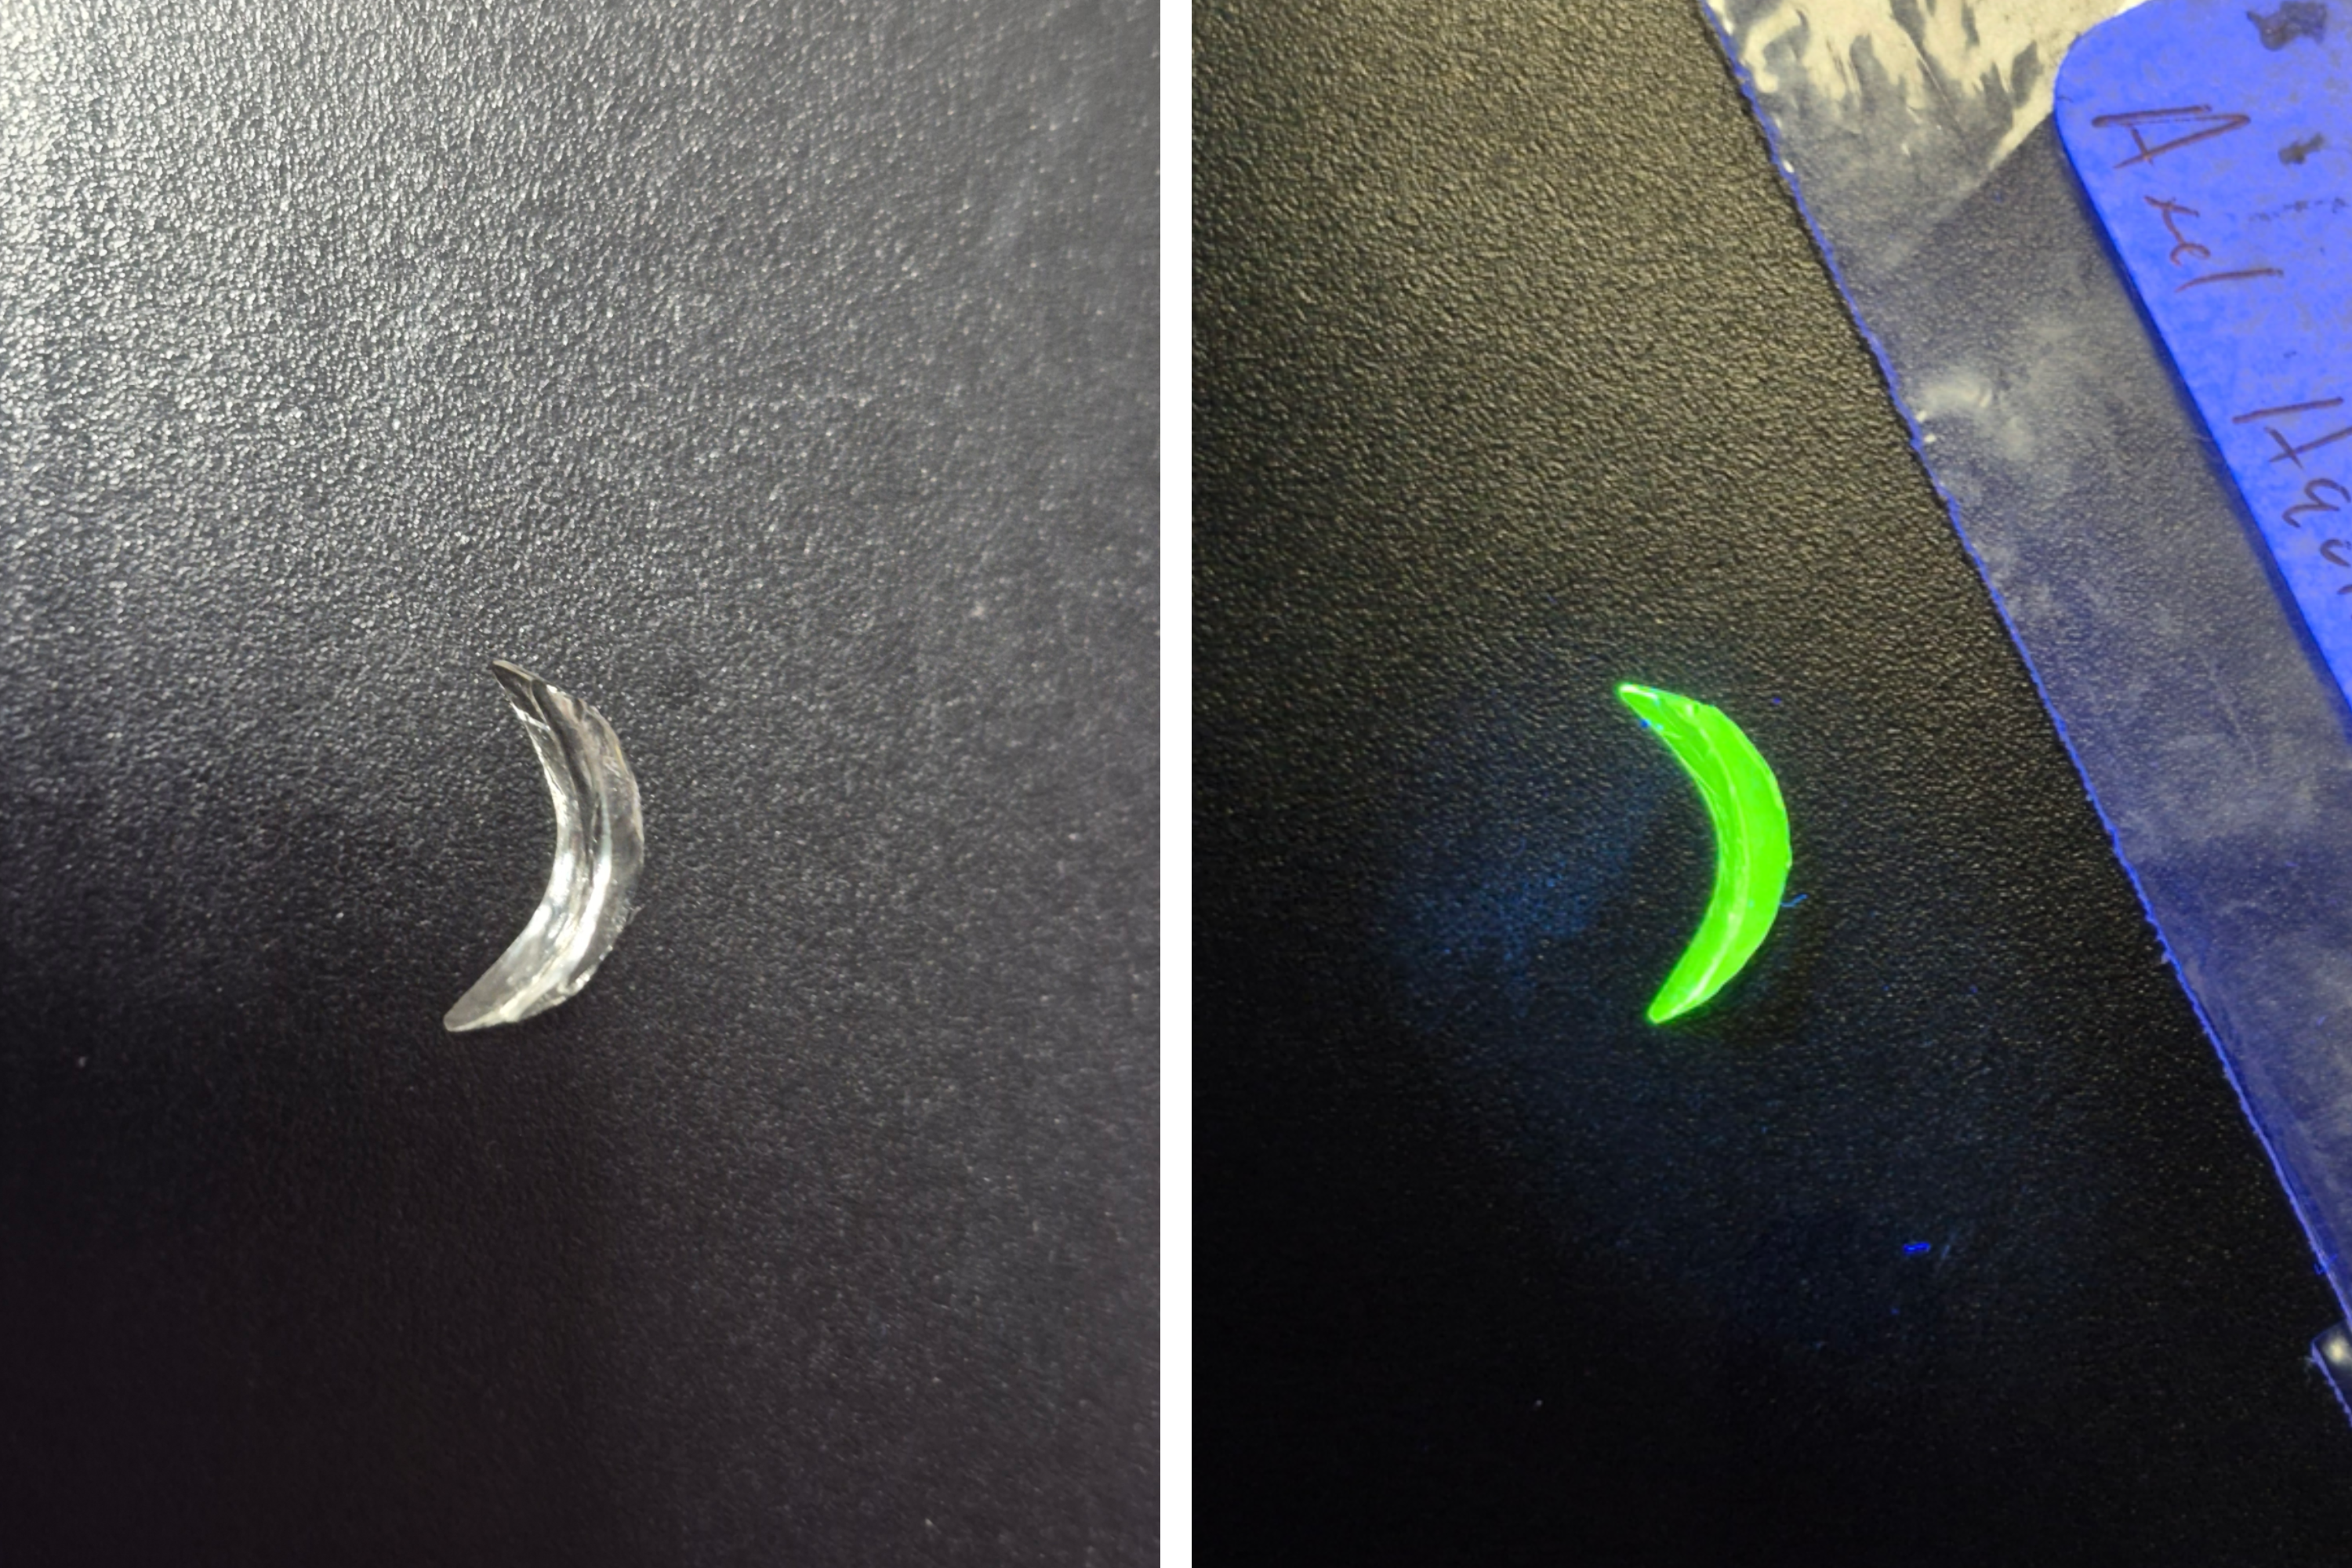
\includegraphics[
        width=\linewidth,
        height=0.22\textheight,
        keepaspectratio
    ]{figs/Tb-fotos.png}

    \captionof{figure}{
        Muestra de Li$_2$B$_4$O$_7$:Tb$_4$O$_7$
        (composición molar: $98\%$, $2\%$).
        A la derecha presenta el fenómeno de fotoluminiscencia;
        excitado con una luz de $366$ nm.
    }
    \label{fig:Tb-fotos}
\end{minipage}